\documentclass{entry}

\title{ハニーポットによる不正ファイルの入手と分析}
\author{G984822019}{吉村 直将}
\supervised{
	\supervisor{教授}{蓑原 隆}
	\supervisor{助手}{田島 信行}
}

\newenvironment{comment}{\color{red}}{\color{black}}

\begin{document}
\maketitle

\section{はじめに}
%\subsection{研究背景}
% 近年,サイバー攻撃の発生件数が年々増加してきており,その攻撃手法も多様化している.
% 対策として,攻撃者を誘き寄せ,
% 不正アクセスを受けるハニーポットを運用し,
% 攻撃者の情報を収集してきた.過去の研究では,
% ハニーポットを利用して,
% ログイン試行時に使われるIDやパスワード,
% ログイン後に攻撃者から送られるシェルコマンド等の情報を収集し,研究を行ってきた.
% 得られる情報の中でログイン後に送られるコマンドを解析することは、
% 攻撃者がログイン成功後にどうゆう意図で,何を目的をとして攻撃を行なってくるかの予測が立てらる.
% 又,コマンドから攻撃者がダウンロードさせようとしてくる不正なソフトウェアの情報を知り、調査できる為,
% より最新の攻撃に対して具体的なセキュリティ対策につながると思われる.

近年,サイバー攻撃の発生件数が年々増加してきており,その攻撃手法も多様化して
いる.
多様化した新しい攻撃に対処するためには攻撃手法の分析が必要である.
攻撃手法の分析のために,  
攻撃者を誘き寄せ,
不正アクセスを受けるハニーポットを用いて
攻撃者の情報を収集
する方法がある.
例えば
ハニーポットを利用して,
ログイン試行時に使われるIDやパスワード,
ログイン後に攻撃者から送られるシェルコマンド等の情報を収集
する方法が提案されている\cite{Entry}.

%ハニーポットは,攻撃を受け,攻撃内容を記録する.その攻撃手法を分析することで,
%攻撃への対策を強化することやデータ収集方法を改良することにつながる.



% 本研究では、ログイン後に攻撃者から送られるコマンドに着目する.
% コマンドについて解析することは、
% 攻撃者がログイン成功後にどうゆう意図を持ち,何を目的をとして攻撃を行なってくるかの予測が立てらる.
% 又,コマンドから攻撃者がダウンロードさせようとしてくる不正なソフトウェアの情報を知り、調査できる為,
% より最新の攻撃に対して具体的なセキュリティ対策につながると思われる.

本研究では,より具体的な攻撃者の攻撃手法の情報を得るため,攻撃者がログイン成功後に行う攻撃に着目し,
ハニーポットを用いて,攻撃者から送信されるコマンドやそのコマンドから入手できるファイルの情報を収集し,解析するシステムを構築する.
そして,攻撃の分析を行い,最新の攻撃内容について警告を発することを目的とする.

\section{攻撃収集分析システム}


攻撃者がダウンロードさせようとしてくる
不正なソフトウェアの解析を実現する為のシステムの構成を図\ref{fig:system}に示す.

\begin{figure}[htbp]
	\centering
 	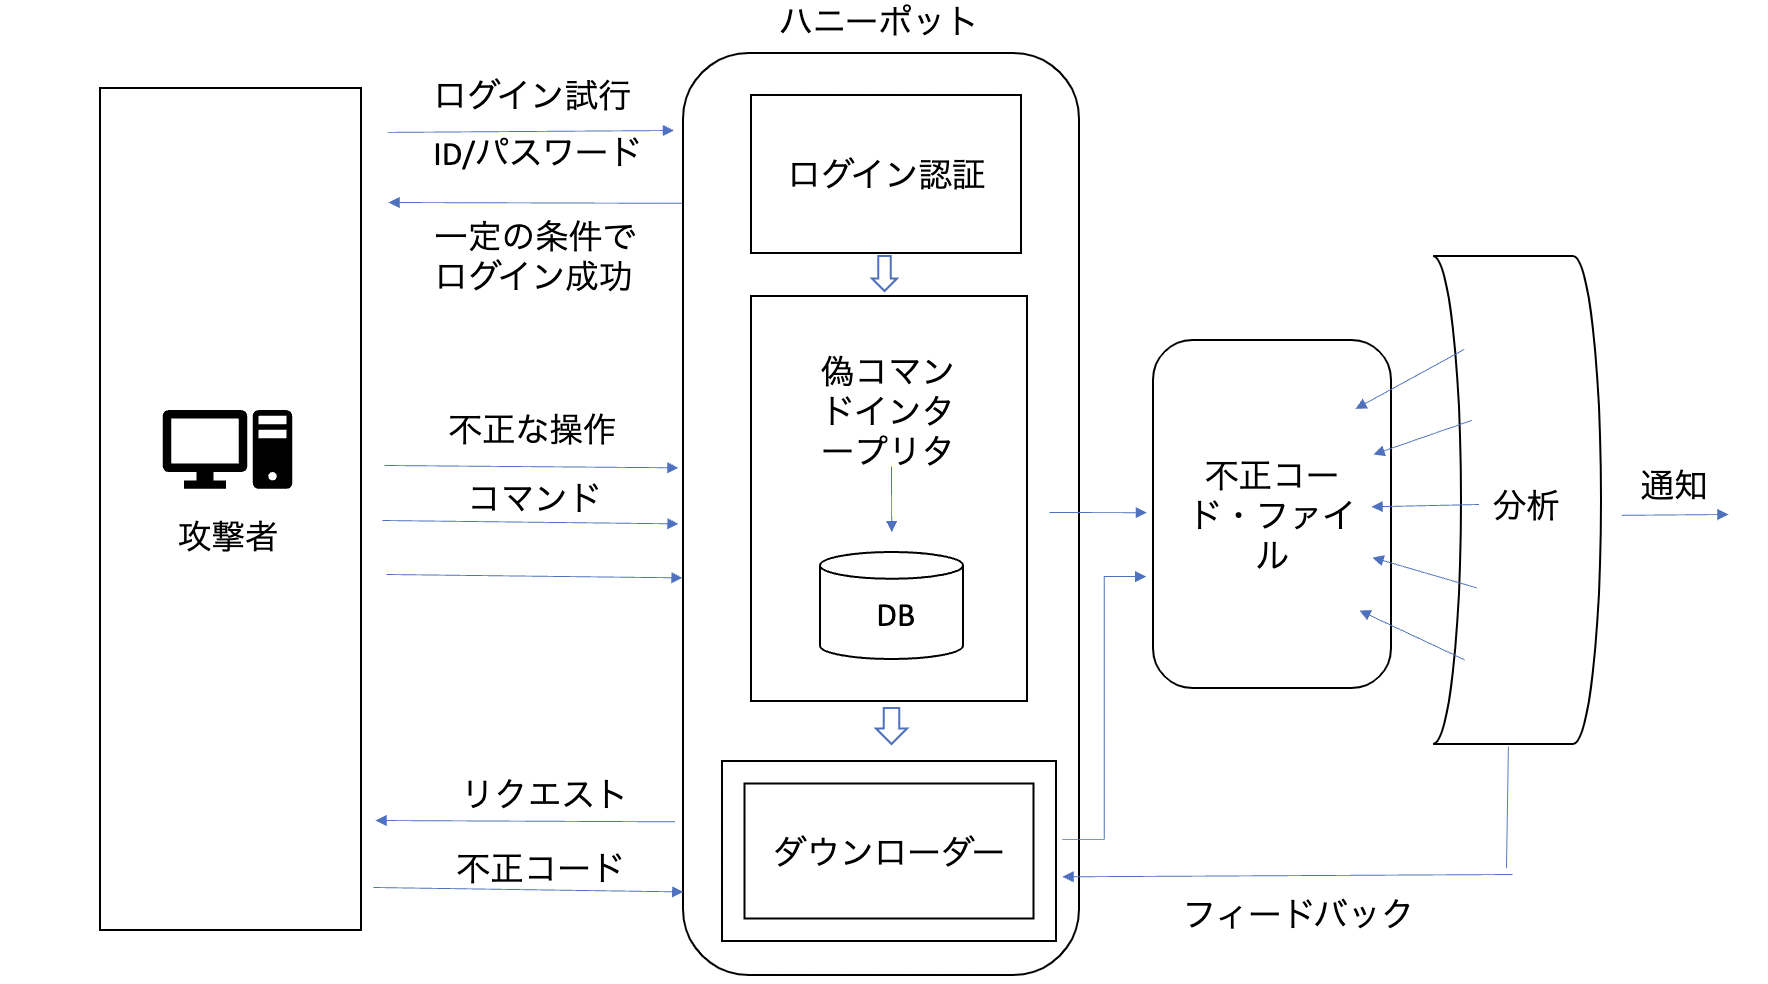
\includegraphics[width=\linewidth]{hpsystem2.png}
 	\caption{システムの構成}\label{fig:system}
\end{figure}



%\subsection{攻撃ホストからハニーポットへの攻撃の流れ}

%攻撃者ホストからハニーポットへの攻撃の流れとして図1に示してある.

% \Repl{攻撃ホスト}{ハニーポット}
% は
% ログイン試行としてID/パスワードを送信してくる
% \Repl{ハニーポットはそれ}{攻撃ホスト}
% に対して,ログイン許可をしている風に見せる.
% \Repl{}{このとき,}ログイン試行時に使われるIDやパスワード
% \Repl{}{を記録する}.

% 攻撃者はログイン\Repl{後}{に成功したシステムを}操作する
% \Repl{為}{ため}に,コマンドを送信する
% \Repl{この攻撃の中でハニーポットはログイン後に}{ので,}
% 攻撃者から送られるシェルコマンド等の情報を収集
% \Repl{し,収集した情報から攻撃手法の研究してきた.}{する}.

ハニーポットは,攻撃者からの何度かのログイン試行を受け,
一定の条件で,攻撃者にログイン成功したと思わせる.
その後,攻撃者にコマンドインタープリタの様な返答を見せ,
不正な操作のコマンドをデータベースDBに収集する.

収集したコマンドから,
攻撃者が不正なサイトから
ダウンロードさせ
ようとする
不正なファイルを安全に入手する.
また,コマンドの中には,コマンドからハニーポット内に
直接不正なファイルを作成しようとしてくるものもあ
るので,安全にファイルを作成して収集する.

収集した不正ファイルのコードから,
どの様な不正ファイルかを分析し警告を発
する.また,
その情報からダウンローダーに生かせるものをフィードバック
する.


% \begin{figure}[htbp]
% 	\centering
% 	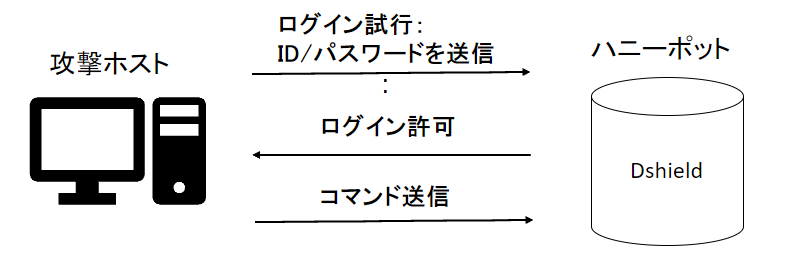
\includegraphics[width=\hsize]{honeypot1.png}
% 	\caption{攻撃の流れ}
% \end{figure}

%\subsection{目的}

% 本研究では,ハニーポットDshieldを用いる.DShield(Distributed Intrusion Detection System)は,
% グローバルなセキュリティコミュニティによって構築された分散型侵入検知システムである.
% 世界中のネットワーク上で発生するセキュリティイベントのデータを収集し,
% 分析することでセキュリティの脅威情報を提供する.Dshieldは研究室で以前から運用していたが,
% ログイン試行時のIdやパスワードを収集することを目的としたハニーポットであった.
% 本研究では,ログイン後のコマンドを収集することが目的としている為,
% 新しくハニーポットを構築することとする.                

%\subsection{システムの実装}

本研究でのハニーポットの実装は,Dshield(Distributed In-trusion Detection System)
と呼ばれる
グローバルなセキュリティコミュニティによって構築された分散型侵入検知システム
をベースに開発を行う.
%世界中のネットワーク上で発生するセキュリティイベントのデータを収集し,
%分析することでセキュリティの脅威情報を提供する.
これまで研究室では主に
攻撃頻度の時系列解析のために
Dshieldハニーポットを利用している\cite{nishida2022}.

図\ref{fig:system}のログイン認証部,コマンドインタープリタ部は,Dshieldの
cowrie に必要な機能を追加する形で実現する.
また,コマンドからファイル又は,URLなどを取集する
ダウンローダー部,
不正ファイルの分析部は,新しく
プログラムを作成する.
% 研究計画として,
% \begin{enumerate}
%     \item Dshieldを運用できる環境を構築をする.
%     \item コマンドを収集するために、Dshieldのプログラム内で、
% 	攻撃者からのコマンドに対してどのような動作をしているかを確認する.
%     \item 実際にDshieldを運用してみる.
%     \item取集したコマンドの内容について調べる.
%     \item 
%     \item ファイルがどのようなものなのか調べる.
% \end{enumerate}
% という手順で進めていき,攻撃ファイルがどの様なものなのか把握し,
% どのような対策が有効的なのか等の警告を発することで,セキュリティの向上に貢献していく.

\section{進捗状況}

Raspberry PiにDshieldをインストールし,パスワードや接続する無線LANの設定を行なった.
Rassberry Piのファイアウォールの設定からSSHを有効にする事で,
外部からの接続をcowrieが対応するように設定した.
また,研究室内のネットワークからの接続は攻撃と見さないように設定した.

%\subsection{Dshieldが行う攻撃者のログイン試行への対処方法}

%Dshieldは研究室で以前から運用されていたがidやパスワードの収集を目的として使われていた.
攻撃者から
コマンドを収集
するために
Dshieldのプログラム
を調査し,
コマンドを収集できているのか確認した.
調査の結果,Dshieldは
攻撃コマンドを取集し,
/srv/cowrie/var/log/cowrieの場所に保存
していることが分かった.

また,ログイン試行に対応しているプログラムが
/src/cowrie/core/の場所にあるauth.pyである
ことを突き止め,解読したところ,
Dshieldは外部からの攻撃者
%(一つの決まったIPアドレス)
からのログイン試行を1回以上のランダム数行うと,
ログイン可能とする
ように設定されていることが
分かった.

% そのログイン成功時に使用していた
% ユーザーIDとパスワードがそのIPアドレス限定でのログイン成功するものとなる.
% これは,ハニーポットと見破られないように考えられたシステムだと思われる.

%\subsection{収集したコマンド内容と攻撃者の意図}
実際にハニーポットを運用し5/19から5/30の期間中にコマンドを取集した.
収集したコマンドの中には
特定のパターンのコマンドが多く発見された.
例えば組み込みLinuxで複数のコマンドをまとめるために使われる
busyBoxが含まれていて,
この期間中に多くの攻撃が組み込みLinuxの機器を対象としていることが分かった.
また,収集したコマンド中には,不正なファイルをダウンロードさせるための
コマンドとしてwgetやcrulにURLを指定したもの
や不正なファイルをハニーポット内に作成するコードを用いたコマンドが見られた.


\section{今後の予定}

9月までにダウンローダー部を完成させ,不正ファイルを取得できるようにする.
その後,収集したファイルの分析を行う部分を作成し,11月までにシステムの運用評価を行う.


\bibliographystyle{entry}
%\bibliographystyle{junsrt}
\bibliography{sample}

\end{document}
